% !TEX root =  ../../Krantz_style.tex

%Having described HSLDA and given details on how to do inference in it, we turn to demonstrations of using HSLDA to solve problems from  two different domains: predicting medical
%diagnosis codes from hospital discharge summaries and predicting product
%categories from Amazon.com product descriptions.

%In the section we describe the application of HSLDA for prediction
%in two hierarchically structured domains. Firstly, we describe using
%discharge summaries to predict diagnoses, encoded as ICD-9 codes.
%Discharge summaries are documents that are authored by clinicians
%to summarize the course of a hospitalization. ICD-9 codes are used
%mainly for billing purposes to indicate the conditions for which a
%patient was treated. Secondly, we describe using Amazon.com product
%descriptions to predict product categories.

\subsection{Hospital Discharge Summaries and ICD-9 Codes}

 Despite the growing emphasis on meaningful
use of technology in medicine, many aspects of medical record-keeping
remain a manual process. In the US, diagnostic coding for billing and insurance
purposes is often handled by professional medical coders who must
explore a patient's extensive clinical record before assigning the
proper codes. %So while electronic health records (EHRs) should be
%adopted by most medical institutions within the next several years,
%largely due to the provisions of HITECH under the American Recovery
%and Reinvestment Act \cite{Blumenthal2009}, there has been little
%movement forward in automating medical coding.


%Similarly, viewing the distribution of topics over discharge summaries
%may reveal information about the latent structure of clinician documentation.
%Lastly, the SLDA model would provide a novel approach to dealing with
%the problem of high dimensionality when representing narrative text
%in a vector space specifically by reducing dimensions from an entire
%vocabulary of potentially tens of thousands of words to a set of several
%dozen topics.

A specific example of this involves labeling of hospital discharge summaries.  These summaries are authored by clinicians to summarize patient
hospitalization courses. They typically contain a record of patient
complaints, findings and diagnoses, along with treatment and hospital course.  The kind of text one might expect to find in such a discharge summary is illustrated by this made-up snippet
\begin{quote}
{History of Present Illness: Mrs. Carmen Sandiego is a 62-year-old female with a past medical history significant for diabetes, hypertension, hyperlipidemia, afib, status post MI in 5/2010 and cholecystectomy in 3/2009.  The patient presented to the ED on 7/11/2011 with a right sided partial facial hemiparesis along with mild left arm weakness.  The patient was admitted to the Neurology service and underwent a workup for stroke given her history of MI and many cardiovascular risk factors ...}
\end{quote} 
For each hospitalization, trained medical coders review the information in the
discharge summary and assign a series of diagnoses codes. Coding follows the
ICD-9-CM controlled terminology, an international diagnostic classification for
epidemiological, health management, and clinical
purposes.\footnote{http://www.cdc.gov/nchs/icd/icd9cm.htm}  These ICD-9 codes are organized in a rooted-tree structure, with each
edge representing an is-a relationship between parent and child, such that the
parent diagnosis subsumes the child diagnosis. For example, the code for
{}``Pneumonia due to adenovirus'' is a child of the code for {}``Viral
pneumonia,'' where the former is a type of the latter.  A representative sub-tree of the ICD-9 code tree is shown in Figure \ref{fig:diagnosis_tree}. It is worth noting that
the coding can be noisy. Human coders sometimes disagree~\cite{Challenge07},
tend to be more specific than sensitive in their
assignments~\cite{Birmetal2005}, and sometimes make
mistakes~\cite{FarzandipourEtAl10}.


\begin{figure}[t]
%tbp] %  figure placement: here, top, bottom, or page
\centering 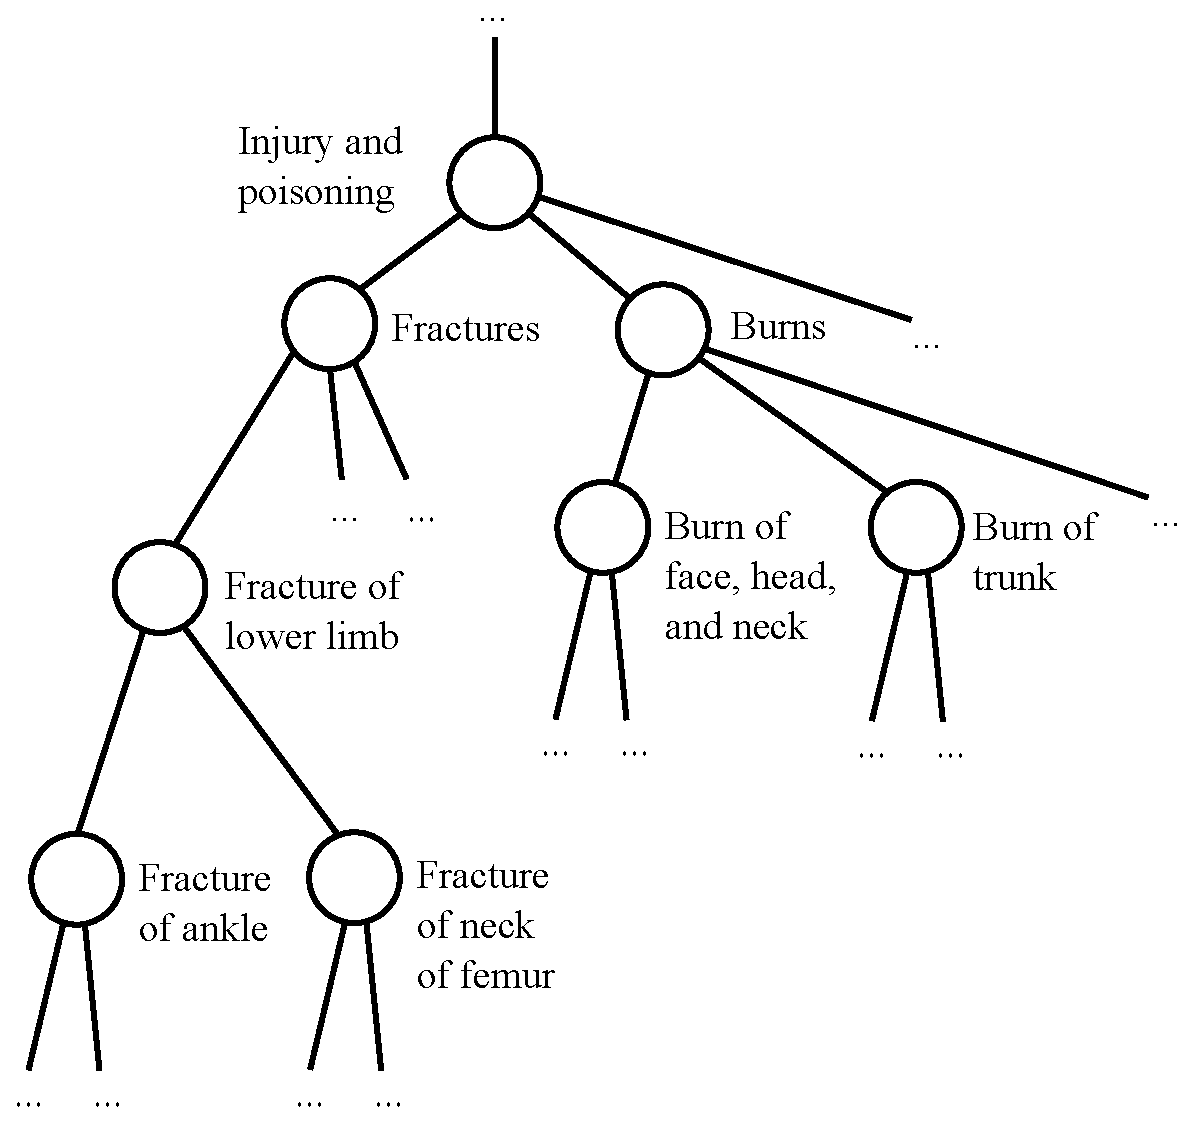
\includegraphics[scale=0.4]{Chapters/chapter1/figures/hi_quality_ICD9_tree_cropped} \caption{An illustration of a portion of the ICD9 hierarchy.}
\label{fig:diagnosis_tree}
\end{figure}


An automated process would ideally produce a more complete and accurate
diagnosis lists. %Also, this model will reveal information about the
%medical records themselves. For example, we may gain an understanding
%of what a specific code actually means in terms of clinical narratives.
The task of automatic ICD-9 coding has been investigated in the clinical
domain.  Methods used to solve this problem (besides HSLDA) range from applying manually derived coding rules
rules to applications of online rule learning approaches \cite{Crammer2007,Goldstein2007,Farkas2008}.
Many classification schemes have been applied to this problem: K-nearest
neighbor , Naive Bayes, support vector machines, Bayesian Ridge Regression, as
well as simple keyword mappings, all with promising
results~\cite{LarkeyCroft95,RibeiroNeto2001,PakhomovEtAl06,Lita2008}.%Ruch2008 omitted

%Much of the work was triggered by the 2007 medical NLP community
%challenge~\cite{Challenge07}.
%The data in the challenge, however, differs from 
%ours in its scope. The datasets were smaller (1,000 training and 1,000 testing
%documents) and focused on radiology reports with a restricted number of ICD-9
%codes (45 of them, compared to 7K+ in our dataset). 

The specific dataset we report results for in this chapter was gathered from the NewYork-Presbyterian Hospital clinical data warehouse. 
It consists of 6,000 discharge summaries and
their associated ICD-9 codes (7,298 distinct codes overall), representing a portion of
the discharges from the hospital in 2009. All included discharge summaries had associated ICD-9 Codes.
Summaries have 8.39 associated ICD-9
codes on average (std dev=5.01) and contain an average of 536.57 terms after
preprocessing (std dev=300.29). We split our dataset into 5,000 discharge
summaries for training and 1,000 for testing.

The text of the discharge summaries was tokenized with
NLTK.\footnote{http://www.nltk.org} A fixed vocabulary was formed by taking
the top 10,000 tokens with highest document frequency (exclusive of names,
places and other identifying numbers). The study was approved
by the Institutional Review Board and follows HIPAA (Health
Insurance Portability and Accountability Act) privacy guidelines.

Here HSLDA is evaluated as a way to understand and model the relationship between a discharge summary and the ICD-9 codes that should be assigned to it.  We show promising results for automatically assigning ICD-9 codes to hospital discharge records.  

%For each hospitalization there are usually several ICD-9 codes assigned
%for billing purposes. These codes are known to be quite specific but
%not very sensitive \cite{}. Regardless of that fact,
%this is one of the only sources for information on patient diagnoses
%aside from the free text. %Aside from prediction, one of the goals is to compare the sensitivity of predictions from the HSLDA model in comparison to the codes in a case where a test closer to ground truth is available. For this we will compare whether predictions for the ICD-9 code associated with anemia are better predicted by HSLDA or by the ICD-9 codes. Anemia was chosen because hemoglobin values are readily available and the definition of anemia according the World Health Organization is approximately 12.5, with a threshold of 12 for women and 13 for men [citation].

\subsection{Product Descriptions and Catalogs}

Many web-retailers store and organize their catalog of products in a
mulitply-rooted hierarchy in addition to providing textual product descriptions 
for most products. Products can be discovered by users
through free-text search and product category exploration. Top-level
product categories are displayed on the front page of the website and lower
level categories can be discovered by choosing one of the top-level categories.
Products can exist in multiple locations in the hierarchy.


\begin{figure}[t]
%tbp] %  figure placement: here, top, bottom, or page
\centering 
\includegraphics[scale=0.4]{Chapters/chapter1/figures/hi_quality_product_tree_cropped} \caption{An illustration of a portion of the Amazon product hierarchy.}
\label{fig:product_tree}
\end{figure}


Amazon.com is one such retailer.  Their product categorization data is available as part of the 
 Stanford Network Analysis Platform (SNAP) dataset~\cite{SNAP}.    A representative sub-tree of the amazon.com DVD product category tree is shown in Figure \ref{fig:product_tree}.  
Product descriptions were obtained separately from the
Amazon.com website directly. Once such description is
\begin{quote}
{Winner of five Academy Awards, including Best Picture and Best Director, The Deer Hunter 
is simultaneously an audacious directorial conceit and one of the greatest films ever made 
about friendship and the personal impact of war. Like Apocalypse Now, it's hardly a conventional 
battle film--the soldier's experience was handled with greater authenticity in Platoon--but its 
depiction of war on an intimate scale packs a devastatingly dramatic punch ... }
\end{quote}
We study the collection of DVDs
in the product catalog specifically.
%We were able to deduce the structure of the
%hierarchy for the Amazon.com products because all ancestors in the
%hierarchy were included with each category label. For example, {}``DVD / Genres
%/ Science Fiction \& Fantasy / Classic Sci-Fi'' is a single product category 
%for the DVD, {}``The Time Machine.''
The resulting dataset contains 15,130 product descriptions for training and 1,000
for testing. The product descriptions consist of
91.89 terms on average (std dev=53.08). Overall, there are 2,691 unique categories.
Products are assigned on average 9.01 categories (std dev=4.91). The vocabulary
consists of the most frequent 30,000 words omitting stopwords. 

HSLDA is used here to understand and model the relationship between the product text description and the products' positioning in the product hierarchy.  We show how to automatically situate a product in a hierarchal product catalog.  


\subsection{Comparison Models}

We compare HSLDA to two closely related models. The comparison models are SLDA with independent
regressors (hierarchical constraints on labels ignored,  i.e. the regression is not conditional) and HSLDA fit by first
performing LDA then fitting probit regressors that respect the conditional label hierarchy (rather than jointly inferring the topics and the regression coefficients). These models were
chosen because they are the strongest available competitors and because they  highlight several pedagogical aspects of HSLDA including performance in the
absence  of hierarchical constraints, the effect of the combined inference, and
regression performance attributable solely to the hierarchical constraints.

SLDA with independent regressors is the most salient comparison model
for our work. The distinguishing factor between HSLDA and SLDA is the
additional structure imposed on the label space, a distinction that in developing HDSLA we
hypothesized would result in a difference in predictive performance. 

 The second comparison model, HSLDA fit by performing LDA first
followed by performing inference over the hierarchically constrained label
space, does not allow
the responses to influence the topics inferred by LDA.
Combined inference has been shown to improve performance in SLDA
\cite{BleiMcAuliffe2008}. This comparison model does not examine the value of utilizing the structured nature 
of the label space, instead it highlights the benefit of combined inference over both the
documents and the label space. 

%The last comparison model is HSLDA with fixed and randomly selected regression
%parameters. There is a baseline benefit that the structure in the label space 
%provides for the prediction of labels. This comparison model is intended to
%quantify the contribution of the structure alone.

For all three models, particular attention was given to the settings of the 
prior parameters for the regression coefficients. These parameters implement an
important form of regularization in HSLDA. In the setting where there are no
negative labels, a Gaussian prior over the regression parameters with a
negative mean implements a prior belief that missing labels are likely to be
negative. Thus, we show model performance for all three models with a
range of values for $\mu$, the mean prior parameter for regression coefficients 
($\mu\in\left\{ -3,-2.8,-2.6,\ldots,1\right\}$).

The number of topics for all models was set to $K=50$, the prior distributions of
$p\left(\alpha\right)$, $p\left(\alpha^{\prime}\right)$, and
$p\left(\gamma\right)$ were all chosen to be gamma with a shape parameter of 1 and a
scale parameter of 1000.   Different values of $K$ corresponding to different numbers of topics were explored, however, the results that we show in the following are not substantially changed in character.  As is usual in mixed-membership models, there is an ideal number of topics that should be used for out-of-sample prediction tasks, however, a full model-selection search varying topic cardinality was not performed for these datasets.

\begin{figure}[h]
\begin{center}
%\subfloat[][\label{fig:1a}]{\includegraphics[width=.49\textwidth]{figs/amazon_pred_varying_mu}}
\subfigure[Clinical data performance.]{\label{fig:1a}\includegraphics[width=.48\textwidth]{Chapters/chapter1/figs/clin_pred_varying_mu}}
%\subfloat[][\label{fig:1c}]{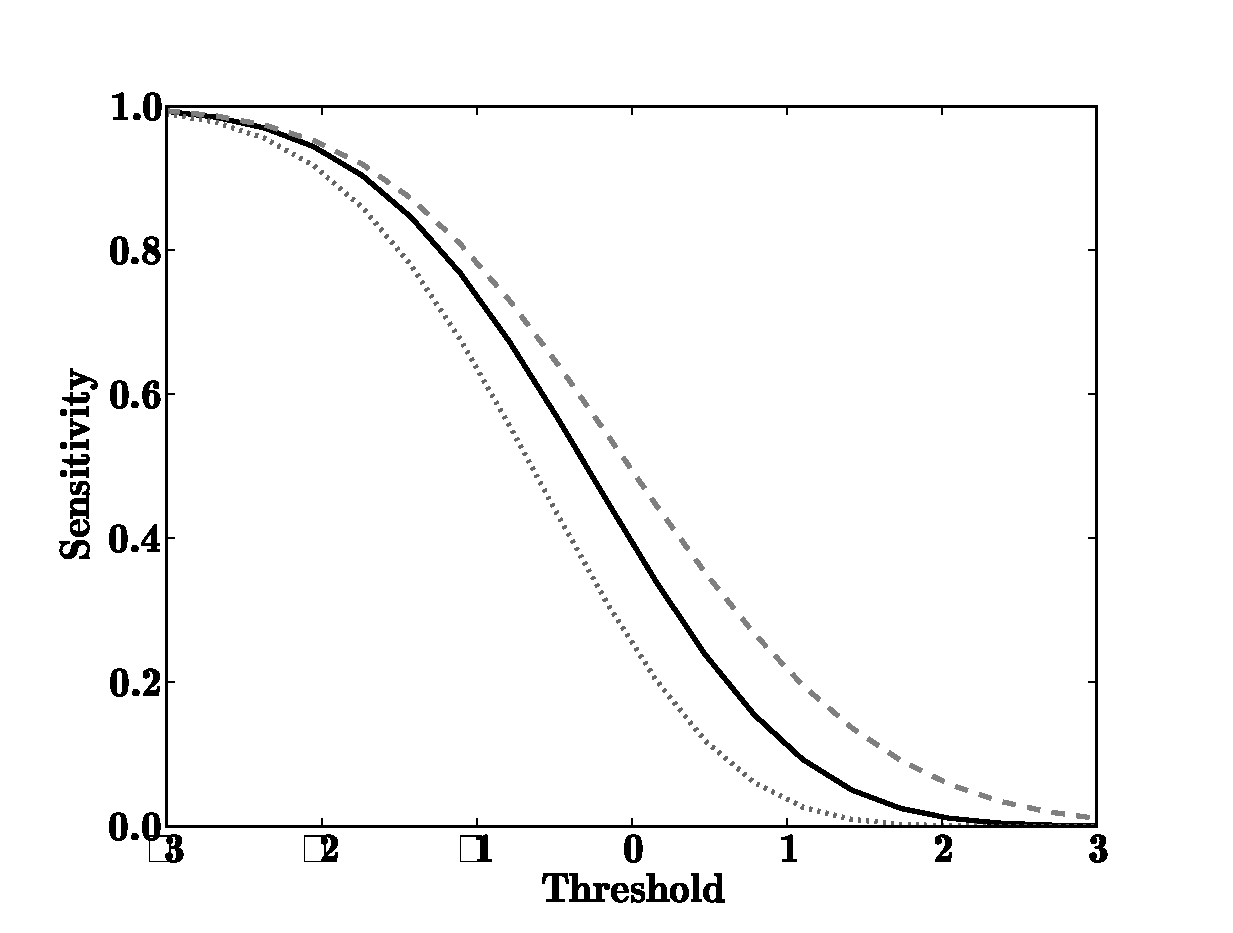
\includegraphics[width=.49\textwidth]{figs/sens_comparison_leafs}}
\subfigure[Retail product performance.]{\label{fig:1b}\includegraphics[width=.48\textwidth]{Chapters/chapter1/figs/amazon_pred_varying_mu}}
%\subfigure[][]{\label{fig:clinical_roc}\includegraphics[scale=0.4]{figs/ROC_comparison_leafs}}
\caption{ROC curves for HSLDA out-of-sample label prediction varying $\mu$, the prior mean of the regression parameters. 
In both figures, solid is HSLDA, dashed are independent regressors + SLDA (hierarchical 
constraints on labels ignored), and dotted is HSLDA fit by running LDA first then running 
tree-conditional regressions.}
%\label{fig:main_results}
\end{center}
\end{figure}


\subsection{Evaluation and Results}

%Outline:
%1. Model evaluation goal, metrics
%2. Gold standard(s), properties
%3. Method for prediction w/ details
%4. Discussion of results
%5. Connection of results with contribution and generality etc

We are particularly interested in
predictive performance on held-out data. Prediction performance was measured
with standard metrics -- sensitivity (true positive rate) and 1-specificity
(false positive rate). 

In each case the gold standard for testing was derived from the test data. To make the comparison as antagonistic to HSLDA as possible (relative to the other models), in evaluation only, ancestors of
observed nodes in the label hierarchy were ignored, observed nodes were
considered positive and descendants of observed nodes were assumed to be
negative. Note that this is different from our treatment of the observations during inference where we marginalize over possible settings of unobserved labels.
For instance, as the SLDA model does not enforce hierarchical
label constraints, when we consider only observed nodes we penalize HSLDA.  This is because
 the is-a hierarchical constraints say that the ancestors of positively labeled nodes must also be positive which the SLDA model cannot guarantee.
Another antagonism of this gold standard is that it is likely to inflate the number of false positives because
the labels applied to any particular document are usually not as complete as
they could be.  ICD-9 codes, for instance, are known to lack sensitivity and their use as a
gold standard could lead to correctly positive predictions being labeled as
false positives~\cite{Birmetal2005}.
However, given that the label space is often large (as in our examples) it is a
reasonable assumption that erroneous false positives should not skew results
significantly. 

Predictive performance in HSLDA is evaluated by computing
 \[p\left(y_{l,\hat{d}}\mid w_{1:N_{\hat{d}},\hat{d}}, w_{1:N_d,1:D},  y_{l\in\mathcal{L},1:D}\right)\] 
for each test document $\hat{d}$ for each observed label $y_{l,\hat{d}}$ (given the test document words). For efficiency, the expectation of this
probability distribution was approximated in the following way. Expectations 
of $\mathbf{\bar{z}}_{\hat{d}}$ and $\boldsymbol{\eta}_l$ were estimated with samples
from the posterior. Fixing these expectations, we performed Gibbs sampling over
the hierarchy to acquire predictive samples for the documents in the test set.
The true positive rate was calculated as the average expected labeling for
gold standard positive labels. The false positive rate was calculated 
as the average expected labeling for gold standard negative labels.

As sensitivity and specificity can always be traded off, we examined
sensitivity for a range of values for two different parameters -- the prior
means for the regression coefficients and the threshold for the auxiliary
variables.  The goal in this analysis was to evaluate the performance of these
models subject to more or less stringent requirements for predicting positive
labels. These two parameters have important related functions in the model. The
prior mean in combination with the auxiliary variable threshold together encode
the strength of the prior belief that unobserved labels are likely to be
negative. Effectively, the prior mean applies negative pressure to the
predictions and the auxiliary variable threshold determines the cutoff. 
For each model type, separate models were fit for each value of the 
prior mean of the regression coefficients.  This is a proper Bayesian
sensitivity analysis. In contrast, to evaluate
predictive performance as a function of the auxiliary variable threshold,
a single model was fit for each model type and prediction was evaluated
based on predictive samples drawn subject to different auxiliary variable
thresholds. These methods are significantly different since the prior mean
is varied prior to inference, and the auxiliary variable threshold is varied
following inference.
%However, as intended, they both highlight model performance 
%under more or less stringent requirements for predicting positive labels.

\begin{figure}[t]
%tbp] %  figure placement: here, top, bottom, or page
\centering \includegraphics[scale=0.4]{Chapters/chapter1/figs/ROC_comparison_leafs} \caption{ROC curve for out-of-sample ICD-9 code prediction varying auxiliary variable threshold. $\mu = -1.0$ for all three models in this figure.}
\label{fig:results_auxiliary_var} 
\end{figure}


Figure~\ref{fig:1a} demonstrates the performance of the model on the clinical data as an ROC curve varying $\mu$.  For instance, 
a hyperparameter setting of $\mu=-1.6$ yields the following performance:
the full HSLDA model had a 
true positive rate of 0.57 and a false positive rate of 0.13, the SLDA model
had a true positive rate of 0.42 and a false positive rate of 0.07, and the
HSLDA model where LDA and the regressions were fit separately had a true
positive rate of 0.39 and a false positive rate of 0.08. These points are highlighted in Figure~\ref{fig:1a}.  Note that the figure is somewhat misleading because for any one value of $\mu$ HSLDA outperforms the comparison models by a relatively large margin. 

These results indicate that the full HSLDA model predicts more of the the
correct labels at a cost of an increase in the number of false positives
relative to the comparison models.  However, as shown in Figure~\ref{fig:1a}  HSLDA outperforms or no worse than the comparison models across across the full range of specificities.  


Example topics (as word lists) learned for the discharge data are given below.  These word lists are computed by sorting
terms in decreasing order based on their probability under a given topic.

\begin{extract}
\begin{tabular}{|c|c|}
\hline
\textbf{Topic 1} & \textbf{Topic 2} \\ \hline \hline
MASS & WOUND \\
\hline
CANCER & FOOT \\
\hline
RIGHT & CELLULITIS \\
\hline
BREAST & ULCER \\
\hline
CHEMOTHERAPY & LEFT \\
\hline
METASTATIC & ERYTHEMA \\
\hline
LEFT & PAIN \\
\hline
LYMPH & SWELLING \\
\hline
TUMOR & SKIN \\
\hline
BIOPSY & RIGHT \\
\hline
CARCINOMA & ABSCESS \\
\hline
LUNG & LEG \\
\hline
CHEMO & OSTEOMYELITIS \\
\hline
ADENOCARCINOMA & TOE \\
\hline
NODE & DRAINAGE \\
\hline
\end{tabular}
\end{extract}

These topics closely correspond to common clinical concepts, namely, cancers of the thorax and wounds common to diabetics suffering from poor peripheral circulation.  Evaluations of the subject coherence of these topics relative to baselines are ongoing, but early results suggest positive findings similar to those reported for other supervised LDA models.

Figure~\ref{fig:1b} demonstrates the performance of the model on the retail product data as an ROC curve also varying $\mu$. For
instance, a hyperparameter setting of $\mu=-2.2$ yields the following
performance: the full HSLDA model had a true positive rate of 0.85 
and a false positive rate of 0.30, the SLDA model had a true positive
rate of 0.78 and a false positive rate of 0.14, and the HSLDA model where
LDA and the regressions were fit separately had a true positive rate of 0.77
and a false positive rate of 0.16. These results follow a similar pattern to the clinical data. These points are highlighted in Figure~\ref{fig:1b}.

Example topics (as word lists) learned for the amazon.com data are given below.  These word lists were also computed by sorting
terms in decreasing order based on their probability under a given topic.

\begin{extract}
\begin{tabular}{|c|c|}
\hline
\textbf{Topic 1} & \textbf{Topic 2} \\ \hline \hline
SERIES & BASEBALL \\
\hline
EPISODES & TEAM \\
\hline
SHOW & GAME \\
\hline
SEASON & PLAYERS \\
\hline
EPISODE & BASKETBALL \\
\hline
FIRST & SPORT \\
\hline
TELEVISION & SPORTS \\
\hline
SET & NEW \\
\hline
TIME & PLAYER \\
\hline
TWO & SEASON \\
\hline
SECOND & LEAGUE \\
\hline
ONE & FOOTBALL \\
\hline
CHARACTERS & STARS \\
\hline
DISC & FANS \\
\hline
GUEST & FIELD \\
\hline
\end{tabular}
\end{extract}

Figure \ref{fig:results_auxiliary_var} shows the predictive performance of HSLDA 
relative to the two comparison models on the clinical dataset as a function of the auxiliary variable threshold. 
For low values of the auxiliary variable threshold, the models predict labels
in a more sensitive and less specific manner, creating the points in the upper
right corner of the ROC curve. As the auxiliary variable threshold is
increased, the models predict in a less sensitive and more specific manner,
creating the points in the lower left hand corner of the ROC curve. HSLDA with full joint inference outperforms SLDA with
independent regressors as well as HSLDA with separately trained
regression. 

%\begin{figure}[t]
%%tbp] %  figure placement: here, top, bottom, or page
% \centering \includegraphics[scale=0.4]{figs/ROC_comparison_leafs} \caption{ROC curve for Out-of-sample ICD-9 code predictions.}
%\label{fig:clinical_roc} 
%\end{figure}
